\datos{color}{}{}
\subsection{\textit{Crazyflie}}
\textit{Crazyflie}, desarrollado por \textit{Bitcraze AB} y presentado en 2013,
Figura~\ref{crazyflie}, es un nano–cuadricóptero modular y de código abierto
ampliamente utilizado en investigación y docencia. Su reducido tamaño, su arquitectura
flexible y su capacidad para integrar distintos módulos de control lo han convertido en una
plataforma de referencia para el estudio de control reactivo, navegación aérea y comportamientos emergentes en robots aéreos. El sistema integra una unidad inercial,
sensores de flujo óptico, barómetro y un microcontrolador encargado de ejecutar los módulos de
control de bajo nivel. \\

Sus usos principales incluyen la investigación en control distribuido a nivel de enjambre,
sistemas multi-robot, navegación reactiva, aprendizaje por refuerzo y experimentación en entornos interiores. Gracias a su
diseño abierto y a su modularidad interna, \textit{Crazyflie} se ha convertido en una herramienta
habitual en laboratorios de robótica aérea y en proyectos de investigación sobre comportamiento
colectivo. \\

\begin{wrapfigure}{r}{0.38\textwidth}
\centering
\vspace{-10pt}
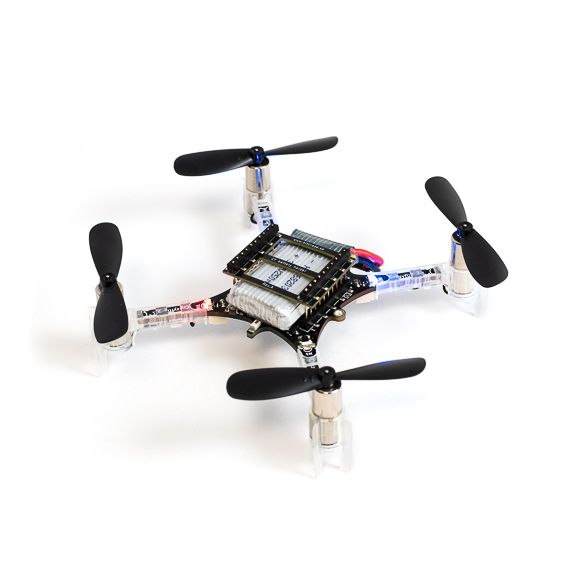
\includegraphics[width=0.34\textwidth]{Images/crazyflie.jpg}
\caption{\label{crazyflie}\textit{Crazyflie 2.1}.}
\vspace{-10pt}
\end{wrapfigure}

\textit{Crazyflie} implementa una arquitectura centralizada, en la que la
información fluye de forma vertical desde los sensores hacia los módulos 
de percepción y estimación, y desde estos hacia los módulos de control que 
generan las órdenes motoras. Un único microcontrolador ejecuta todos los 
niveles funcionales —estabilidad, control de acción, control de altura, 
evasión de obstáculos y estimación del estado—, de modo que ningún sensor 
ni actuador es gestionado de manera autónoma por módulos independientes. 
Estos no constituyen niveles de competencia.\\

\textit{Crazyflie} utiliza un sistema de locomoción aéreo basado en cuatro rotores controlados
de manera independiente. \\

\subsection*{Referencias}
\cite{BitcrazeWebsite} \fullcite{BitcrazeWebsite}. \\
\cite{7989376} \fullcite{7989376}.\\